\section{The Project}
If computers are able to understand text, they might perform better in many settings. Automatic content categorization is a way of determining the meaning of a text, where the text is categorized to the most describing category from a set consisting of desirable categories.
%nderstanding text is important for 
%utomatic content categorization is useful for determining the meaning of a text which is useful in many settings. 
%Given a set of desirable categories it
To be able to categorize articles, it is 

Thus our overall goal is defined as creating a classifier that maps keywords from a predefined keyword list and to one or more pre-defined categories. The automatic categorization will include both the creation of the predefined keyword list and the mapping function, which are both essential for categorizing collections of texts based on their content. 

\begin{figure}[H]
\centering
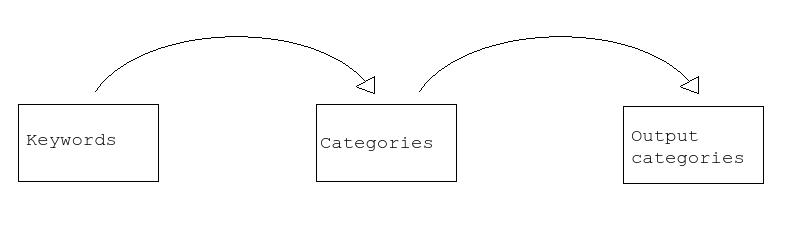
\includegraphics[width=1\textwidth]{Chapters/Introduction/classification_process.jpeg}
\caption{A simplified illustration of the categorization process.}
\label{fig:classification_process}
\end{figure}
%This classifier will be used as part of an automatic categorization process. 
%Our overall goal is therefore to make an automatic categorization that have a predefined keyword list and start by creating a mapping from each keyword to a category from another predefined list. Where the category of a text can be defined from the keywords found in the text. 

\subsection{An Overview of Challenges}
The main challenges encountered had to do with Wikipedia, mainly because the encyclopedia is maintained by thousands of volunteers which also leads to a complicated and complex structure. 

\subsubsection{Encoding}
The titles and categories consists of characters in different languages. 
% INSERT EXAMPLE HERE


\subsubsection{The Structure of Wikipedia}
The underlying structure of Wikipedia is quite complex, which led to 

\subsubsection{Creating a mapping to desirable output}
